\documentclass[t, 11pt]{beamer}
\pdfmapfile{+sansmathaccent.map}
%%% Работа с русским языком
\usepackage{cmap}				
\usepackage{mathtext} 				
\usepackage[T2A]{fontenc}		
\usepackage[utf8]{inputenc}			
\usepackage[english,russian]{babel}	

\usetheme{Ilmenau}
\usecolortheme{lily} % Цветовая схема

\usepackage{xcolor} % подкрашивать текст

%%% Работа с картинками
\usepackage{graphicx}

\usepackage{csquotes}

\hypersetup{				
	colorlinks=true,       	
	linkcolor=blue,          
	citecolor=blue,       
	filecolor=magenta,      
	urlcolor=magenta           
}


\title{Chatbots}
%\subtitle{topic modeling}
%\author{Чувакин Сергей}
\date{25.11}
%\institute[<<Анализ больших данных в бизнесе, экономике и обществе>>]{<<Высшая школа экономики>>}
\institute{<<Высшая школа экономики>>}
\begin{document}
	\frame[plain]{\titlepage}
	\section{Outline}
	
	\begin{frame}
		\frametitle{\insertsection} 
		\begin{block} {}
			 
			\hyperlink{l1}{\beamerbutton{Чатботы}}
		\end{block}
			\begin{block}{}
		\hyperlink{l2}{\beamerbutton{Task-oriented}}
		\end{block}
				\begin{block}{}
		\hyperlink{l2}{\beamerbutton{Other}}
		\end{block}
	\end{frame}
	

\subsection{Chatbots} \label{l1}
\begin{frame}
	\frametitle{\insertsection}
	\frametitle{\insertsubsection}  
	Chatbots are small computer programs used to simulate the method of human conversation and interact with real people automatically to help them with their issues and complete their tasks.
	\begin{itemize}
		\item Button/Menu-Based Chatbots
		\item Keyword-Based Chatbots
		\item Natural Language Processing Chatbots
	\end{itemize}
\end{frame}


\begin{frame}
	\frametitle{\insertsection}
	\frametitle{\insertsubsection}  

	\begin{itemize}
\item Потребность человека в общении (болталка Алисы)
\item Интерфейс приложения
\item Голосовое управление (Siri, Alexa, Алиса)
	\end{itemize}
\end{frame}


\subsection{Task-oriented} \label{l2}


	\begin{frame}
	\frametitle{\insertsection}
	\frametitle{\insertsubsection}
		\begin{itemize}
\item О чём люди должны спрашивать чатбота?
\item Какие интенты внутри поддерживаемых доменов бот должен
обрабатывать?
\item Какие сущности могут быть в каждом сценарии? Какие
ограничения?
\item Как будут обрабатываться ошибки?
\item Как будут обрабатываться неподдерживаемые домены?
\item Что будет, если на бота будут материться? Оскорблять? Приставать?
\item Проработка персонажа.
	\end{itemize}	
\end{frame}





\begin{frame}
	\frametitle{\insertsection}
	\frametitle{\insertsubsection}
	
	\begin{itemize}
		\item Open domain — чатбот умеет поддерживать разговор на любую
		тему.
		\item Closed domain — чатбот умеет поддерживать беседу на
		ограниченное количество тем. 
	\end{itemize}
	
\end{frame}





\begin{frame}
	\frametitle{\insertsection}
	\frametitle{\insertsubsection}
	

Диалог vs. беседа


Диалог — единичная реализация сценария.
Беседа = диалог + диалог + диалог


Поддержка состояний — когда бот запоминает предыдущие
реплики человека. Это можно делать как в рамках одного
диалога, так и в рамках всей беседы.

\end{frame}


\begin{frame}\
	\frametitle{\insertsection}
	\frametitle{\insertsubsection}
	
	
	%\vspace{1cm}
	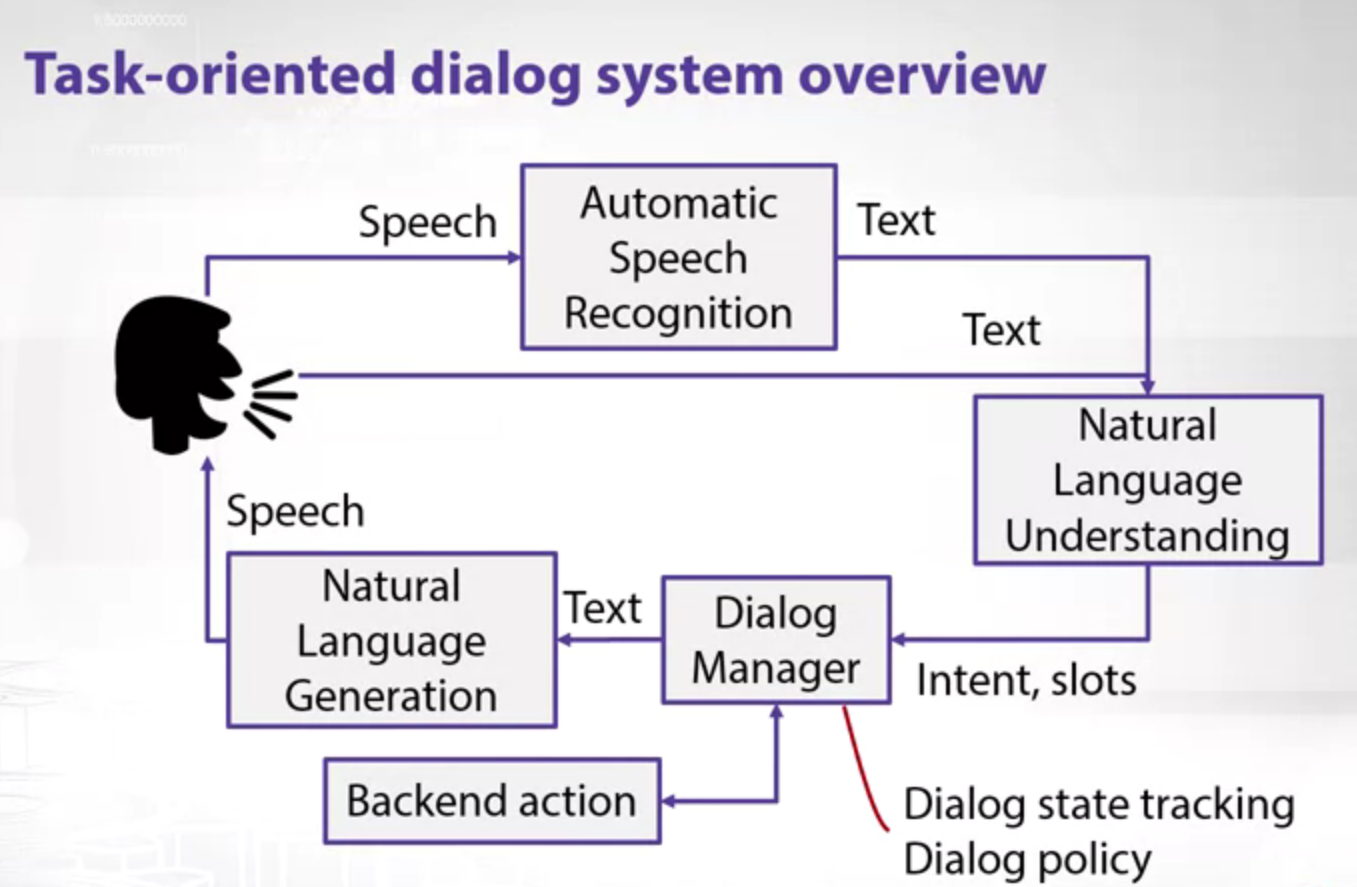
\includegraphics[width=0.8\linewidth]{whole_system.png}
	
	
	
	
\end{frame}






\begin{frame}\
	\frametitle{\insertsection}
	\frametitle{\insertsubsection}
	Откуда брать ответы?
	
	\begin{itemize}
		\item Retrieval-based
		\item Generative-based
	\end{itemize}
\end{frame}

\begin{frame}\
	\frametitle{\insertsection}
	\frametitle{Retrieval-based}
	
	
	
	Как ответить?
	
	\begin{itemize}
		\item Распознать интенцию 
		\item Подготовить формы ответов со слотами для заполнения 
		\item Заполнить форму
	\end{itemize}
	
	
\end{frame}


\begin{frame}\
	\frametitle{\insertsection}
	\frametitle{Retrieval-based}
	
	
	
	Пример формы:
	
- Я хочу взять билет на самолёт из \textcolor{blue}{Москвы} в \textcolor{blue}{Лиссабон} на \textcolor{blue}{1
ноября}.


- Билет из \textcolor{blue}{Москвы} в \textcolor{blue}{Лиссабон} на \textcolor{blue}{1 ноября} будет стоить \textcolor{blue}{13 000
рублей}.
	
\end{frame}

\begin{frame}\
	\frametitle{\insertsection}
	\frametitle{Retrieval-based}
	
	
	
	Как распознать интенцию? 
	
	\begin{itemize}
		\item Пдойдет любая модель на веторизованных текстах (bow, tf-idf, n-grams) - baseline
		\item RNN (LSTM, GRU)
		\item CNN (предпочтительно)
	\end{itemize}
	
	
\end{frame}

\begin{frame}\
	\frametitle{\insertsection}
	\frametitle{Retrieval-based}
	
	
	
	Как найти метки? 
	
	\begin{itemize}
		\item regex
		\item CRF
		\item RNN (seq2seq)
		\item CNN (seq2seq)
		\item any seq2seq model..
	\end{itemize}
	
	
\end{frame}


\begin{frame}\
	\frametitle{\insertsection}
	\frametitle{\insertsubsection}
	Slot tagging
	
	%\vspace{1cm}
	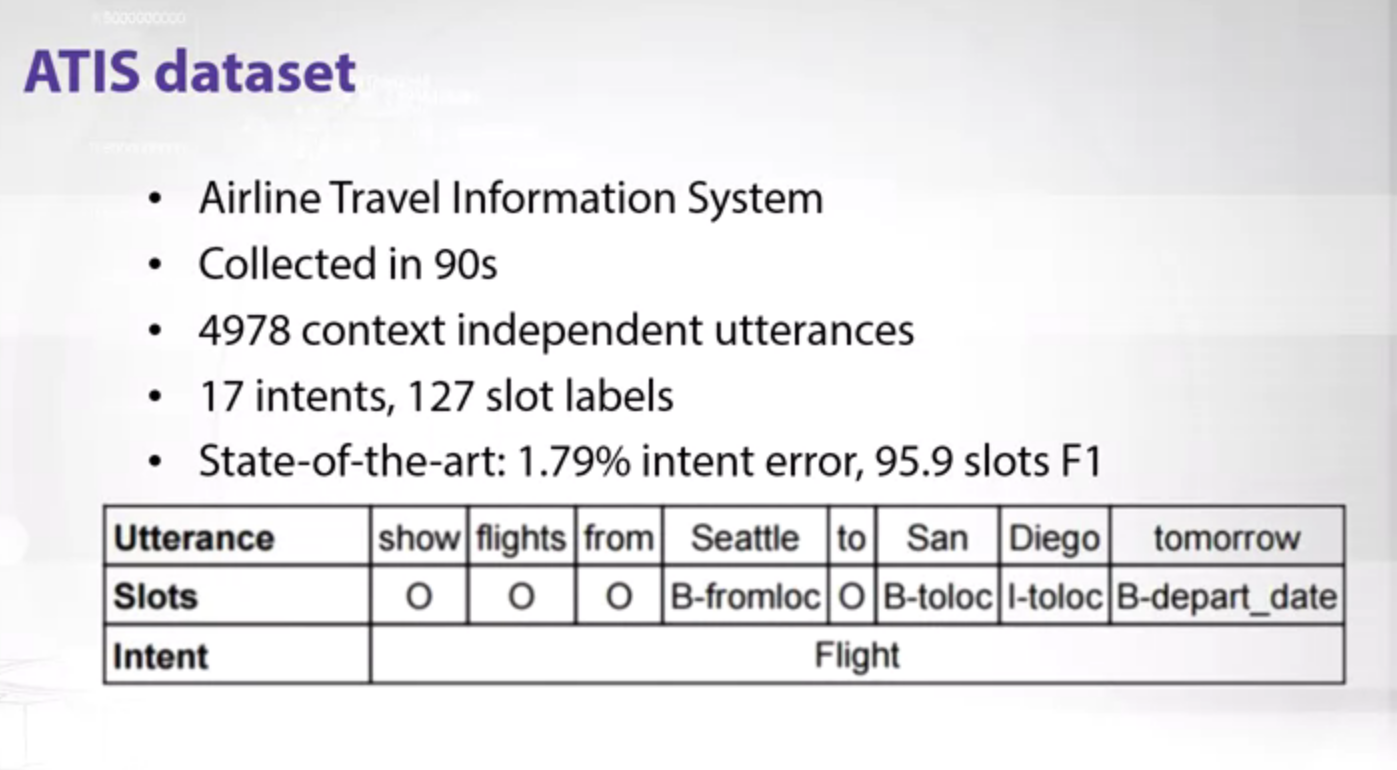
\includegraphics[width=0.9\linewidth]{ex1.png}
	
	
	
	
\end{frame}



\begin{frame}
	\frametitle{\insertsection}
	\frametitle{\insertsubsection}
	Поддерржка состояния:
	
	%\vspace{1cm}
	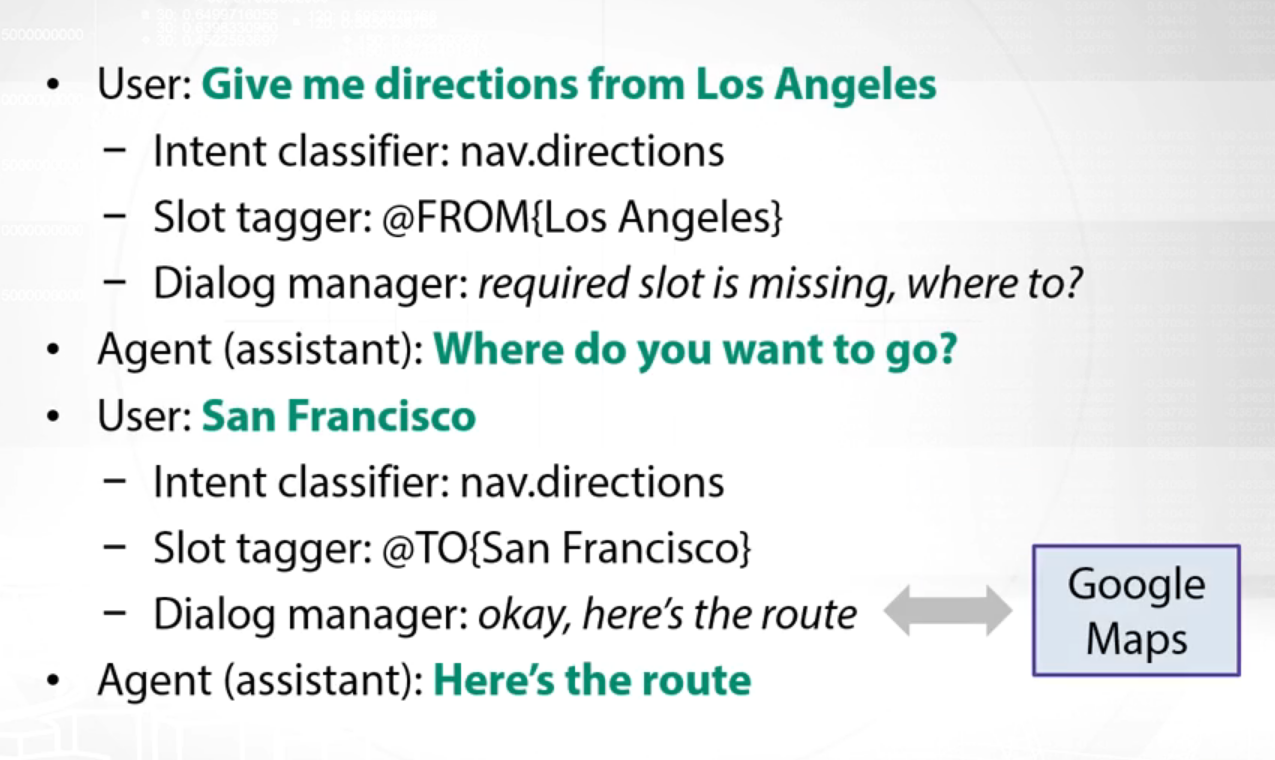
\includegraphics[width=0.9\linewidth]{ex0.png}
	
	
	

\end{frame}




\begin{frame}
	\frametitle{\insertsection}
	\frametitle{\insertsubsection}
	Pipelilne recap:
	\begin{itemize}
		\item domain
		\item intention 
		\item slot tagging 
	\end{itemize}
	
\end{frame}


\subsection{Other} \label{l3}


\begin{frame}
	\frametitle{\insertsection}
	\frametitle{seq2seq-нейросети}
   
   
   
Нейросеть вида ”sequence to sequence” принимает на вход
некоторую последовательность чего угодно (чисел, пикселей,
символов) и порождает другую последовательность чего угодно,
сооветствующую первой. Нас скорее интересуют
последовательности букв или слов, хотя в отдельных случаях в
качестве токенов используются целиком вопросы и ответы.
	
\end{frame}

	
	
	
\begin{frame}
	\frametitle{\insertsection}
	\frametitle{seq2seq-нейросети}
	Как реализовать?
	
	\begin{enumerate}
\item Берём обучающий корпус запросов и ответов.
\item Тренируем рекуррентную (LSTM или GRU) нейросеть, которая
принимает на вход последовательность токенов запроса и
выдаёт в качестве ответа некую другую последовательность
токенов.
\end{enumerate}
\end{frame}



\begin{frame}
	\frametitle{\insertsection}
	\frametitle{seq2seq-нейросети}
	Когда мы можем такое делать?
\begin{itemize}
\item Есть много данных.
\item Мы уверены в качестве используемых данных.
\item Нет ресурсов на разработку правил.
\item Чатбот скорее развлекательный.
\item Нам не очень жалко свою репутацию.
\end{itemize}
\end{frame}

%
%\begin{frame}
%	\frametitle{\insertsection}
%	\frametitle{\insertsubsection}
%	
%	
%	%\vspace{1cm}
%	u
%	
%%	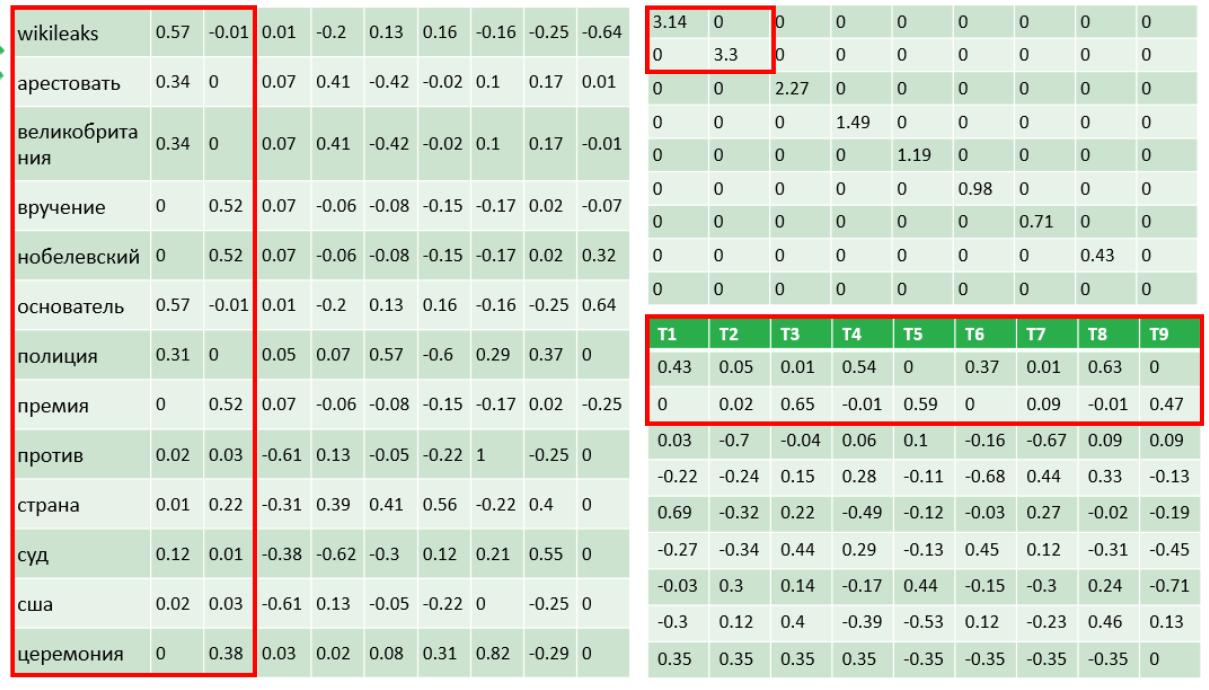
\includegraphics[width=0.9\linewidth]{deux.png}
%	
%	
%	
%
%\end{frame}



%	\begin{frame}
%	\frametitle{\insertsection}
%	\frametitle{\insertsubsection}  
%	Синонимы кватификаторов 
%	\begin{center}
%		\begin{table}[]
%			\begin{tabular}{c|c|c}
%				\hline
%				Синоним &Расшифровка &Квантификатор \\
%				\hline
%		+ & 1 и более раз &\{1,\}   \\
%		* & 0 и более раз &\{0,\}   \\
%
%		? &  0 или 1 раз& \{0,1\}  \\
%  
%			\end{tabular}
%		\end{table}
%	\end{center}
%\end{frame}

%\begin{frame}
%	\frametitle{\insertsection}
%	\frametitle{\insertsubsection}  
%	Чтобы убрать жаность необходимо добавить ?
%	
%	\vspace{0.5cm}
%	
%	Строка на вход  <<( dfghvb ) sdvsd ( sdcvkjnh ) sdvsd ( dkjhvgr ) sdvfv.>>
%	
%	\vspace{0.5cm}
%	
%	шаблон: r"$\backslash$(.+?$\backslash$)"
%	
%	\vspace{0.5cm}
%	
%	на выходе: ['dfghvb', 'sdcvkjnh', 'dkjhvgr']
%	
%\end{frame}



%	\begin{frame}
%	\frametitle{\insertsection}
%	\frametitle{\insertsubsection}
%	
%	
%	\vspace{1cm}
%	\includegraphics[width=0.9\linewidth]{page2.png}
%	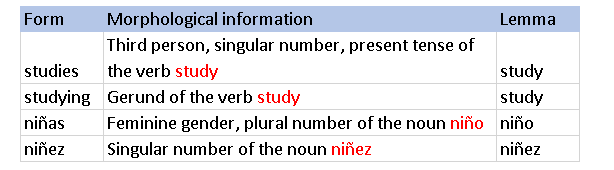
\includegraphics[width=0.7\linewidth]{lem.png}
%\end{frame}
\end{document}